\documentclass[handout]{beamer}

\usepackage{fontspec} 
% \usepackage{lsp-makros}
\useoutertheme{lsp}

\usepackage{lsptitle}
\usepackage{tikz}
\usetikzlibrary{positioning}
\usepackage{multicol}
\usetikzlibrary{fit}
\def\two@digits#1{\ifnum#1<10 0\fi\number#1}
\def\mytoday{\two@digits{\number\day}.\two@digits{\number\month}.\number\year}


\usepackage{xspace,multicol}
\newcommand{\latex}{\LaTeX\xspace}


\newcounter{lastpagemainpart}
\footnotesep0pt
\renewcommand{\footnoterule}{}
\usefootnotetemplate{
  \noindent
  \insertfootnotemark\insertfootnotetext}

\let\beamerfn=\footnote
\renewcommand{\footnote}[1]{%
\let\oldfnsize=\footnotesize%
\let\footnotesize=\tiny%
\beamerfn<\thebeamerpauses->{#1}%
\let\footnotesize=\oldfnsize}


\date{2023-06-28}

\usepackage{eurosym}  
 
\renewcommand{\centerline}[1]{\hfill#1\hfill\hfill\mbox{}}


\title{Open Text Collections}
% \institute{}
\author[Nordhoff]{Sebastian Nordhoff\\Corpus Glosés: de la construction à l'exploitation automatique}



\begin{document}
\lspbeamertitle




\section{intro}
\frame{
\frametitle{Introduction}
%   \includegraphics[height=.2\textheight]{./path/to/graphicsfile}
  
\includegraphics[width=.5\textwidth]{jldc2008.png}%
  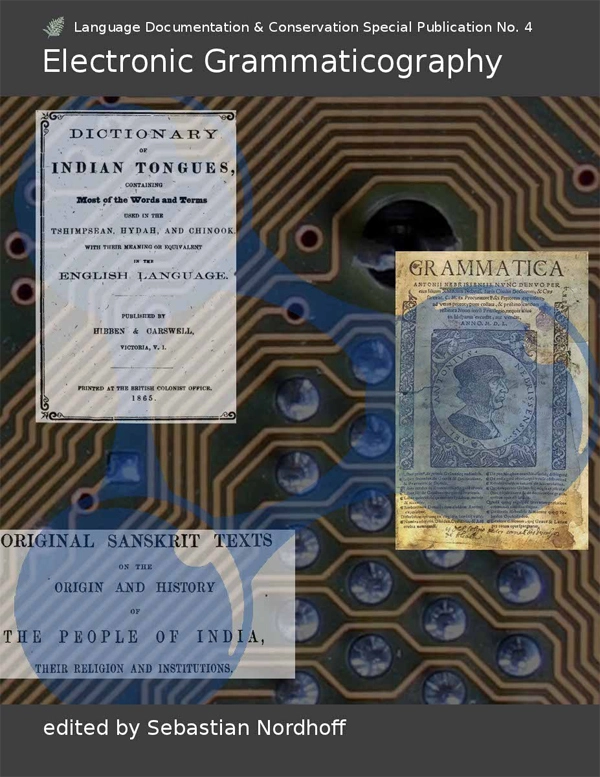
\includegraphics[height=.5\textheight]{ldc.png}
  \begin{itemize}
    \item work on grammaticography since 2007
    \item Language Science Press since 2014
    \item starting 2023: open text collections
  \end{itemize}


}


\frame{
\frametitle{Boasian Trilogy:\\ publication options}
%   \includegraphics[height=.2\textheight]{./path/to/graphicsfile}
  \begin{enumerate}
    \item \textbf{Dictionaries}: many outlets
    \item \textbf{Grammatical descriptions}: many outlets
    \item \textbf{Text collections}: no significant outlets
  \end{enumerate}
}

\frame{
\frametitle{Existing platforms}
%   \includegraphics[height=.2\textheight]{./path/to/graphicsfile}
  \begin{itemize}
    \item  \textbf{TILA}: \url{https://www.americanlinguistics.org/?page_id=1830} (closed access)
    \item \textbf{pangloss}: \url{https://pangloss.cnrs.fr/} (eclectic, manual workflow)
    \item \textbf{doreco}: \url{https://doreco.huma-num.fr} (transcribed audio, finished project?)
%     \item eopas:
  \end{itemize}
}

\frame{
\frametitle{Open Text Collections}
%   \includegraphics[height=.2\textheight]{./path/to/graphicsfile}
  \begin{itemize}
    \item Platform to start in 2023
    \begin{itemize}
    \item      open
    \item   prestigious
    \item   interoperable
    \item   start 2023-09-15
    \end{itemize}
  \end{itemize}
}
\section{guiding principles}
\frame{
\frametitle{Guiding principles}
%   \includegraphics[height=.2\textheight]{./path/to/graphicsfile}
  \begin{itemize}
    \item  \textbf{texts}, not audio
    \item  \textbf{edited}, not naturalistic
    \item  \textbf{curated}, not eclectic
    \item \textbf{peer reviewed}, not legacy or opportunistic\medskip
    \item  \textbf{availability first}: no paywalls, registration, waiting times, click rallyes
    \item  \textbf{community}
    \item  \textbf{openness}
    \item  \textbf{prestige}: seasoned editors

  \end{itemize}
}
\section{input}

\frame{
\frametitle{Import}
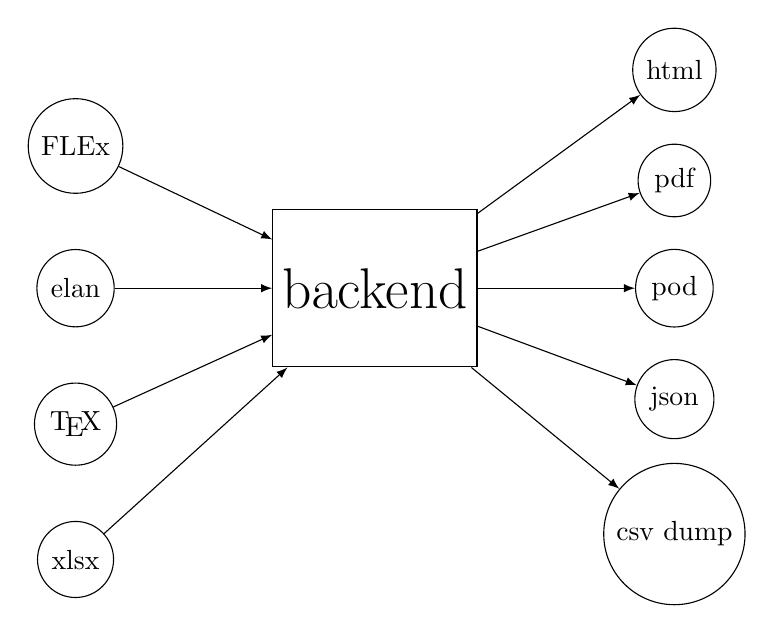
\begin{tikzpicture}
  \node(backend)[rectangle,draw,minimum height=2cm]{\huge backend};
  \node(elan)[circle,draw,left =2cm of backend]{elan};
  \node(flex)[circle,draw,above = 7mm of elan]{FLEx};
  \node(tex)[circle,draw,below = 7mm of elan]{\TeX};
  \node(xlsx)[circle,draw,below = 7mm of tex]{xlsx};
  \node(pod)[circle,draw,right = 2cm of backend]{pod};
  \node(pdf)[circle,draw,above = 4mm of pod]{pdf};
  \node(html)[circle,draw,above =4mm of pdf]{html};
  \node(json)[circle,draw,below = 4mm of pod]{json};
  \node(csv)[circle,draw,below = 3mm of json]{csv dump};
\draw[-latex](elan)->(backend);
\draw[-latex](flex)->(backend);
\draw[-latex](tex) ->(backend);
\draw[-latex](xlsx)->(backend);
\draw[-latex](backend)->(pod);
\draw[-latex](backend)->(pdf);
\draw[-latex](backend)->(html);
\draw[-latex](backend)->(json);
\draw[-latex](backend)->(csv);
\end{tikzpicture}
}


\frame{
\frametitle{Consistency on input files}
  \begin{itemize}
    \item  For a project at ZAS Berlin, I analyzed 20,000 ELAN files culled from various endangered language archives
    \item Take home message: everybody does what they want with ELAN
    \item tier names and structures vary wildly
    \item it is possible to build an API to access glossed material in language archives, but it is painful.
  \end{itemize}
  \includegraphics[width=.5\textwidth]{tiertypetreemap-all.png}
}

\section{backend}

\frame{
\frametitle{Backend}
  \begin{itemize}
    \item CSV for the web (CSVW)
    \item text-based
    \item simple
    \item extensible
    \item easy to version
  \end{itemize}
}

\frame{
\frametitle{CSVW}
  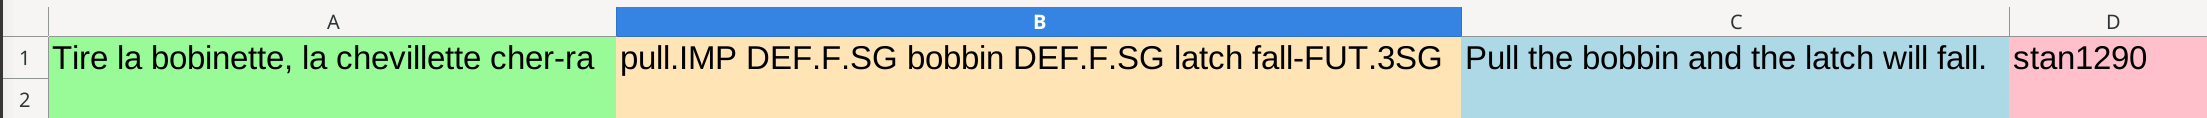
\includegraphics[width=\textwidth]{backend_csv.png}
  \begin{itemize}
    \item three obligatory columns
    \begin{itemize}
      \item vernacular
      \item glosses
      \item translation
    \end{itemize}
    \item can be expanded by further columns as necessary
    \item Leipzig Glossing Rules
    \item correspondences and constraints between cells in the same row
  \end{itemize}

}

\section{output}
\frame{
\frametitle{Output formats}
%   \includegraphics[height=.2\textheight]{./path/to/graphicsfile}
  \begin{itemize}
    \item dump (csv, json-ld, nq, rdf)
    \item pdf
    \begin{itemize}
       \item printed pdf = book
     \end{itemize}
    \item html
    \item query interface
    \begin{itemize}
      \item see \href{imtvault.org}{https://imtvault.org/?q=coconut}
    \end{itemize}
  \end{itemize}
}

\section{workflow}
\frame{
\frametitle{Workflow}
\begin{columns}
\column{4.5cm}
  \begin{itemize}
    \item  every text collection is prepared on GitHub
    \item  DOI via the GitHub-Zenodo bridge
    \item review via GitHub issues
    \item collections approved by the regional boards get a new release (1.0), archived on Zenodo, and are accepted in the relevant Zenodo communities.
  \end{itemize}
\column{5.5cm}
  \includegraphics[width=1.1\textwidth]{zenodo_otc.png}
\end{columns}
}

\frame{
\frametitle{Quality assurance}
%   \includegraphics[height=.2\textheight]{./path/to/graphicsfile}
  \begin{itemize}
    \item technical review (automated, probably via GitHub actions)
    \begin{itemize}
      \item number of words match between vernacular and glosses
      \item number and type of morphemes match between vernacular and glosses
      \item abbreviations are either Leipzig Glossing Rules or listed in separate document
    \end{itemize}
    \item content review
    \begin{itemize}
      \item regional boards with area specialists
      \item precise setup to be debated
      \item can use GitHub Issues
    \end{itemize}
  \end{itemize}
}

\section{technical}
\frame{
\frametitle{Data model}
%   \includegraphics[height=.2\textheight]{./path/to/graphicsfile}

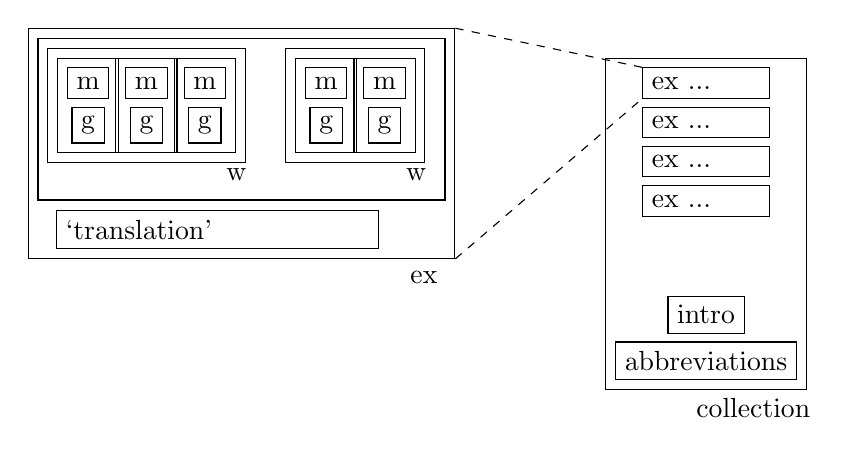
\begin{tikzpicture}
  \node(m1)[rectangle, draw]{m};
  \node(g1)[rectangle, draw, below=1mm of m1]{g};
  \node(mg1)[fit=(m1)(g1), draw] {};

  \node(m2)[right=2mm of m1,rectangle, draw]{m};
  \node(g2)[rectangle, draw, below=1mm of m2]{g};
  \node(mg2)[fit=(m2)(g2), draw] {};

  \node(m3)[right=2mm of m2,rectangle, draw]{m};
  \node(g3)[rectangle, draw, below=1mm of m3]{g};
  \node(mg3)[fit=(m3)(g3), draw] {};

 \node(w1)[fit=(mg1)(mg2)(mg3), draw] {};
 \node(w1label)[below=2mm of g3,xshift=4mm]{w};


  \node(m4)[rectangle, draw,right=of m3]{m};
  \node(g4)[rectangle, draw, below=1mm of m4]{g};
  \node(mg4)[fit=(m4)(g4), draw] {};

  \node(m5)[right=2mm of m4,rectangle, draw]{m};
  \node(g5)[rectangle, draw, below=1mm of m5]{g};
  \node(mg5)[fit=(m5)(g5), draw] {};


 \node(w2)[fit=(mg4)(mg5), draw] {};
 \node(w2label)[below=2mm of g5,xshift=4mm]{w};
 \node(translation)[rectangle, draw, below=6mm of w1,xshift=9mm]{`translation'~~~~~~~~~~~~~~~~~~};

  \node(wblock)[fit=(w1)(w2label), draw] {};

  \node(ex)[fit=(wblock)(translation), draw] {};

 \node(exlabel)[below=15mm of g5,xshift=5mm]{ex};

 \node(ex1)[draw,rectangle,right = 3cm of m5]{ex ... ~~~~~};
 \node(ex2)[draw,rectangle,below = 1mm of ex1]{ex ... ~~~~~};
 \node(ex3)[draw,rectangle,below = 1mm of ex2]{ex ... ~~~~~};
 \node(ex4)[draw,rectangle,below = 1mm of ex3]{ex ... ~~~~~};
 \node(intro)[draw,rectangle,below = 1cm of ex4]{intro};
 \node(abbr)[draw,rectangle,below = 1mm of intro]{abbreviations};
  \node(text)[fit=(ex1)(abbr), draw] {};
\node(w2label)[below=1mm of abbr,xshift=6mm]{collection};

\draw[dashed](ex.north east)--(ex1.north west);
\draw[dashed](ex.south east)--(ex1.south west);


\end{tikzpicture}

}


\frame{
\frametitle{FAIR}
%   \includegraphics[height=.2\textheight]{./path/to/graphicsfile}
  \begin{itemize}
    \item
          \textbf{findable}:
              registered, linked, metadata
    \item
          \textbf{accessible}:
              no paywalls
    \item
          \textbf{interoperable}:
              many different well-defined and open formats
    \item
          \textbf{reusable}:
              open license
  \end{itemize}
}

\section{funding model}

\frame{
\frametitle{Funding}
%   \includegraphics[height=.2\textheight]{./path/to/graphicsfile}
  \begin{itemize}
    \item 3 year grant from DFG, 2023-2026, 1.5 FTE
    \item after that consortial funding via Language Science Press
  \end{itemize}
}
\section{people}
\frame{
\frametitle{People}
%   \includegraphics[height=.2\textheight]{./path/to/graphicsfile}
  \begin{itemize}
    \item
      \textbf{Mandana Seyfeddinipur}, Director ELDP/ELAR at BBAW
    \item
      \textbf{Christian Döhler}, Papuanist, holder of the \textit{Gabelentz Award} for the best published grammar (A grammar of Komnzo)
    \item
      \textbf{Sebastian Nordhoff}, managing director for Language Science Press, extensive experience in Open Access publishing and Linked Data
    \item
        student assistants
  \end{itemize}
}
\frame{
\frametitle{Regional boards}
%   \includegraphics[height=.2\textheight]{./path/to/graphicsfile}
  \begin{itemize}
    \item \textbf{Oceania} Christian Döhler, Kilu von Prince (Düsseldorf)
    \item \textbf{Africa}  Alena Witzlack-Makarevich (Jerusalem), Jeff Good (Buffalo)
    \item \textbf{Eurasia} Michael Rießler (Joensuu)
    \item \textbf{South America} Matt Coler (Groningen), Nick Emle (Groningen)
    \item \textbf{Caucasus} Diana Forker (Jena)
    \item further board probably via cooption
  \end{itemize}
}
\section{content}
\frame{
\frametitle{Planned text collections}
%   \includegraphics[height=.2\textheight]{./path/to/graphicsfile}

\begin{multicols}{2}
\begin{itemize}
    \item Komnzo
    \item Bine
    \item Daakaka
    \item Dalkalaen
    \item Muylaque Aymara
    \item Iquito
    \item two Amazonian languages
    \item Kawesqar
    \item Hinuq
    \item Sanzhi
    \item Chirag Dargwa
    \item  Tabasaran
    \item Gawarbati
    \item Palula
    \item Saek
  \end{itemize}
  \end{multicols}
}

\frame{
\frametitle{Thank you}

\Large Thank you for your attention.
\medskip


\url{http://opentextcollections.org}
\medskip

Mastodon \url{https://fedihum.org/@otc}
\medskip


\url{https://twitter.com/OpenTextColl}

\includegraphics[height=\textheight]{logo.pdf}

}

%\setcounter{framenumber}{\thelastpagemainpart}
\end{document}
